%\subsection{Incremental facility location}
%\label{sec:incremental}

In this section, we consider the setting where facilities might be deployed incrementally, with a fixed capacity. We consider a given schedule $t_0, t_1, \ldots, t_m$, which denote the discrete times at which we want to monitor the epidemic. At time $t_u$, we let $k_u \geq 0$ denote the number of new facilities with uniform capacity $cap_u \geq 1$ that can be deployed. We also $\mathbf{p}(t_u)$ be the demand vector at time $t_u$. In our experiments, $t_1, t_2, \ldots, t_m$ are equidistant and corresponding to the times after $1$ week, $2$ weeks, and so on. Our method \textsc{OnlineKMed} starts with an initial
deployment of $k_0$ facilities at time $t_0$, based on the population density, and at each subsequent time $t_u$ with $u > 0$, it uses the current infection rates to determine the locations where $k_u$ additional facilities could be deployed, \emph{without altering the locations of facilities already deployed}. Let $O_u$ denote the set of open hospital at time $t_u$. We require that $O_0 \subseteq O_1 \subseteq O_2 \ldots \subseteq O_m$.

Let us consider any time $t_u$ where $u > 0$. Let $C_{u-1}$ denote the total capacities of all hospital up to time $t_{u-1}$. The first question is ``how should we determine the number $k_u$ of new hospitals to be built?'' In practice, there are two main factors for estimating parameter $k_u$: (1) our current budget and (2) the forecasted demand vectors $\mathbf{p}(t_v)$ for a few next time points $\{t_v: v \geq u\}$. Indeed we want to cover as many population nodes as possible; however, the total opening cost will have to be bounded by some given budget.

Now suppose we know the value of $k_u$. Then the maximum number of patients who can be served is $C_u = C_{u-1} + k_u \times cap_u$. We have two cases:
\begin{itemize}
	\item Case $C_u \geq |\mathbf{p}(t_u)|_1$: it is possible to serve all patients at time $t_u$. We solve the corresponding capacitated $k$-median instance with the set $O_{u-1}$ being opened and obtain the solution $O_u$. Now the optimal assignment of patients to open facilities in $O_u$ can be easily found by solving a minimum cost max-flow problem.
	
	\item Case $C_u < |\mathbf{p}(t_u)|_1$: it is impossible to serve all patients at time $t_u$. We suggest the following policy. We sort all patients (recall that the node $j \in P$ has $p_j(t_u)$ patients at time $t_u$) in decreasing order of distance to the nearest hospital in $H$. Let $S_u$ be the set of the top $|\mathbf{p}(t_u)|_1 - C_u$ patients in this list. We refer to $S_u$ as the set of ``outliers'' at time $t_u$. We shall need some alternative treatment for the people in $S_u$. Then we exclude $S_u$ from $P$ to obtain a new demand vector $\mathbf{p}'(t_u)$ such that $|\mathbf{p}'(t_u)|_1 = C_u$. The problem can now be solved as in the first case.
	
\end{itemize}








\newpage
\subsection{Our results}
In this section, we summarize our numerical results for the incremental hospital location problem. Recall that $t_1, t_2, \ldots$ are the times after $1$ week, $2$ weeks, etc from the start of the epidemic. We exploit the property of kernel facilities in the following manner: for the first $s-1$ time points (weeks), $t_1, \ldots, t_{s-1}$, we only use the kernel with uniform capacity $cap_1$. Starting from time $t_{s}$, we build $k'$ additional hospitals at time points  $t_s, t_{s+w}, t_{s+2w}, \ldots$ for some $w \in \mathbb{N}$. In other words, we are able to build $k'$ additional facilities after every $w$ weeks starting from time $t_s$. These new hospitals will have uniform capacity $cap_2$.


\begin{itemize}
\item
Figure \ref{fig:online1} compares the incremental solution with 
$s=1$, $w=2$, $k=5, k' = 2$, $cap_1 = cap_2 = 100$, with the static fractional solution
(which serves as a lower bound). We find that the solutions are really close, after about 5 weeks.
\item
The performance of the incremental approach depends on the initial capacity, $cap_1$, as shown
in Figure \ref{fig:online2}. If $cap_1$ is too low, this can cause spikes in the average cost
at some subsequent time, when the patient demand peaks.
\item
Another important determinant for the performance of the incremental algorithm is the
number $k'$ of facilities opened at each time. Figure \ref{fig:online3} compares two different
policies, namely (i) one every two weeks, starting at week 10, and
(ii) two each week, starting week 1. As one would expect the former has a much
higher cost, especially in the early stages of the epidemic.
\end{itemize}

\begin{figure}[h]
  \centering % left bottom right top
    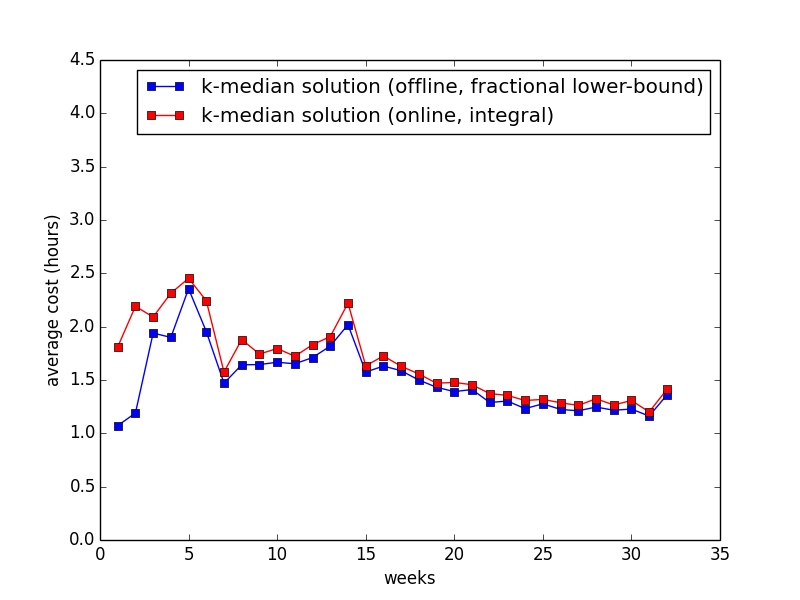
\includegraphics[width=0.30\textwidth]{figs/plot_kmed_CAP100.png}
    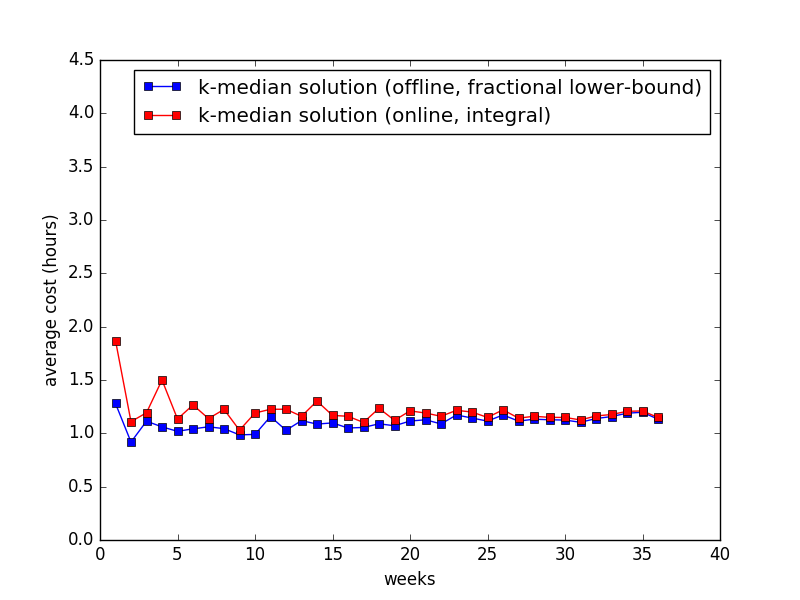
\includegraphics[width=0.30\textwidth]{figs/plot_kmed_CAP100_SL.png}
    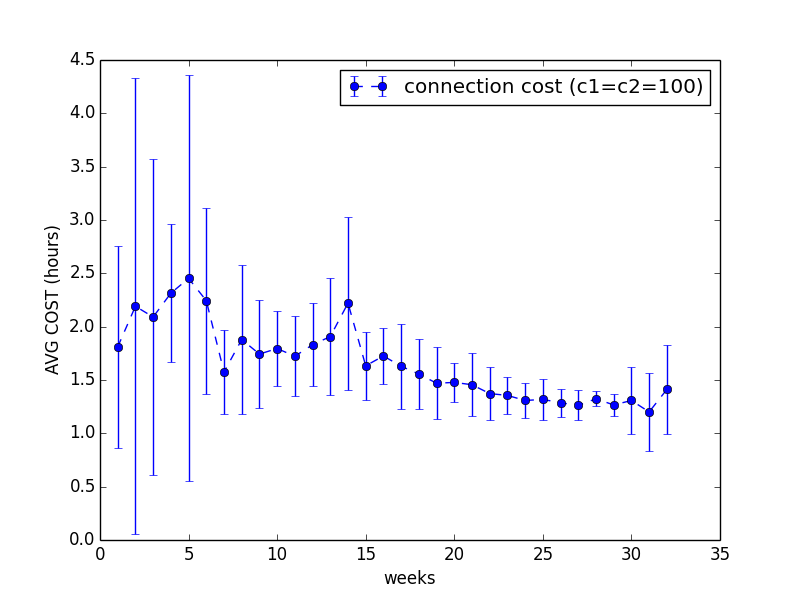
\includegraphics[width=0.3\textwidth]{figs/plot_online_cap100.png}
    \caption{Comparing the static and incremental strategies for
$s=1$, $w=2$, $k=5, k' = 2$, $cap_1 = cap_2 = 100$ for
(a) Liberia, and (b) Sierra Leone.
The variance in the solution costs over multiple iterations is shown in (c).}
\label{fig:online1}
\end{figure}

\begin{figure}[h]
  \centering % left bottom right top
    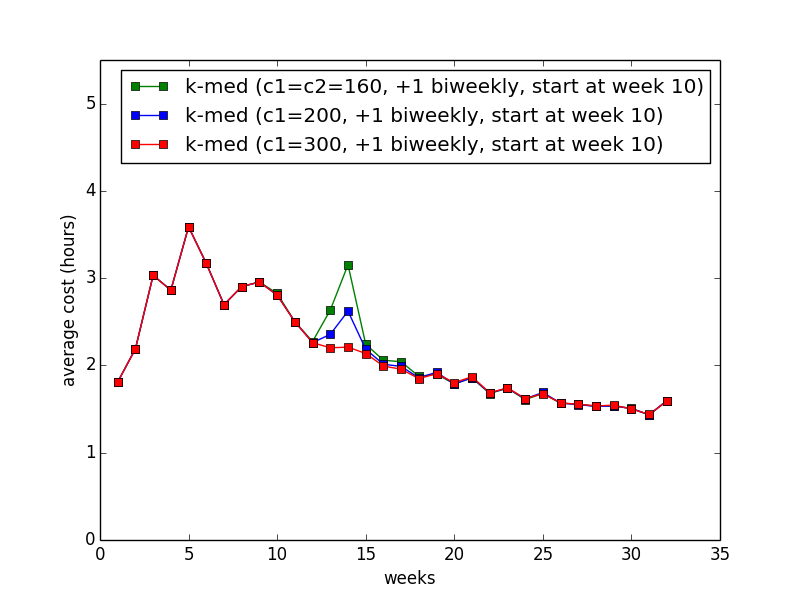
\includegraphics[width=0.45\textwidth]{figs/plot_kmed_c1.png}
    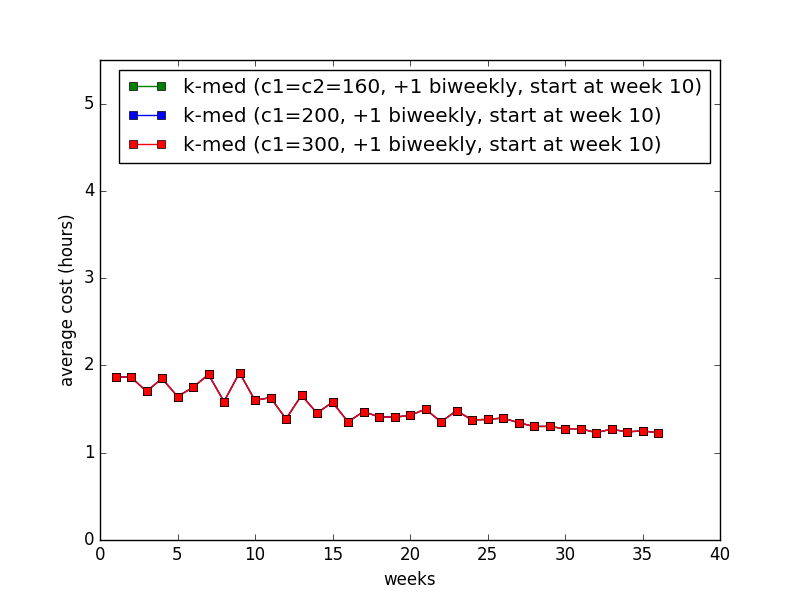
\includegraphics[width=0.45\textwidth]{figs/plot_kmed_c1c2_SL.png}
    \caption{Effect of the initial capacity $cap_1$ on the incremental solution, with
parameters $s = 10, w = 2, k' = 1, cap_2 = 160$, for (a) Liberia, and (b) Sierra Leone.}
\label{fig:online2}
\end{figure}

\begin{figure}[h]
  \centering % left bottom right top
    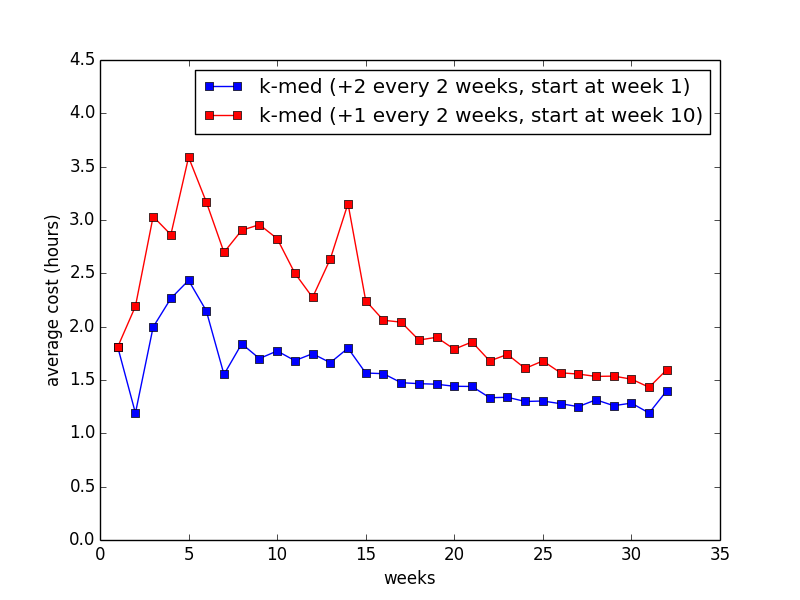
\includegraphics[width=0.45\textwidth]{figs/plot_kmed_CAP160_s1_s10.png}
    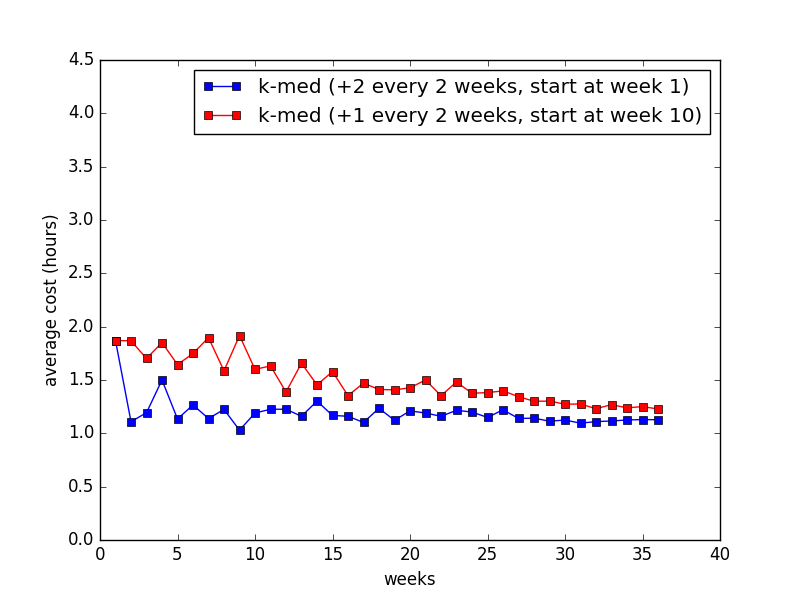
\includegraphics[width=0.45\textwidth]{figs/plot_kmed_CAP160_s1_s10_SL.png}
    \caption{Two different opening policies, with kernel size = $5$, for
(a) Liberia and (b) Sierra Leone.}
\label{fig:online3}
\end{figure}


